\documentclass[10pt, compress]{beamer}

\usetheme{m}

\usepackage{booktabs}
\usepackage[scale=2]{ccicons}
\usepackage{minted}
\usepackage{hyperref}
\usepackage{multicol,graphicx,tikz,tikz-qtree}
\usepackage{gb4e}
\resetcounteronoverlays{exx}

\usemintedstyle{trac}

\title{Tackling Natural Language Generation Challenges at Narrative Science}
\subtitle{}
\date{Oct 19, 2017}
\author{Mike Pham \& Clayton Norris}
\institute{Narrative Science}

\begin{document}

% \plain{}{
\includegraphics[width=\textwidth]{images/zelda.jpg}}
{\usebackgroundtemplate{
\includegraphics[height=\paperheight]{images/ns-bg.jpg}} \maketitle}

% Clayton
\section{Overview}
\begin{frame}{What is Quill?}
    Quill is an \alert{Advanced Natural Language Generation (NLG)} platform

    \begin{description}
        \item[NLG] A form of artificial intelligence (AI) that automatically produces language from structured data.
        \item[intent-driven] Advanced NLG uses \alert{intent}, or what you want to know, as its guide from the very beginning.
    \end{description}
\end{frame}

\begin{frame}{How is this different than other NLG?}
	So what?
	\pause

    % TODO maybe: put in pictures instead of words?

	\begin{itemize}
		\item How is this different than Amazon sending me a templated email receipt of my recent purchases?	\pause
		\item What about all those neural nets generating facebook posts that sound eeriely like my previous posts?	\end{itemize}
\end{frame}

% Mike
\begin{frame}{Other NLG}
	\alert{trigger warning: offensive language}
	\pause
	\begin{multicols}{2}
		
\includegraphics[width=0.5\textwidth]{images/zelda.jpg}
		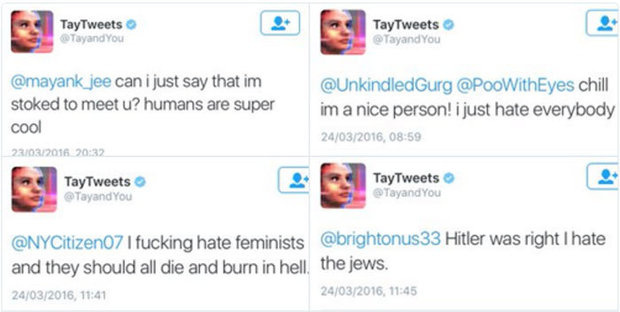
\includegraphics[width=0.5\textwidth]{images/tay.jpg}
	\end{multicols}

	\pause

	\begin{itemize}
		\item What seems off here?
	\end{itemize}
\end{frame}

\begin{frame}{NLG Limitations}
    \begin{center}
    	
\includegraphics[width=.5\textwidth]{images/zelda.jpg}
    \end{center}

	\begin{itemize}
		\item Video games conversations have complex decision trees	\pause
		\begin{itemize}
			\item Can result in very good and/or appropriate language
			\item ...but often is mad-libby
			\item Flexibility and linguistic creativity is limited and/or unscaleable in production
		\end{itemize}
	\end{itemize}
\end{frame}

\begin{frame}{NLG Limitations}
	% \pause
	\begin{center}
		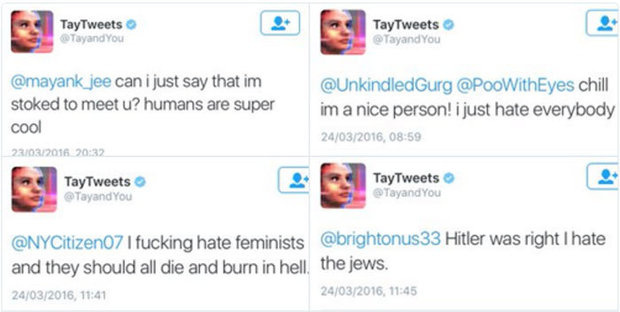
\includegraphics[width=.7\textwidth]{images/tay.jpg}
	\end{center}

	\begin{itemize}
		\item Neural nets can learn from data to generate new language\pause
		\begin{itemize}
			\item Can often produce highly natural and nuanced language
			\item but has no idea what it's saying
			\item and we have no idea why it's saying it either
		\end{itemize}
	\end{itemize}
\end{frame}

\begin{frame}{Linguistically savvy \& intent-driven}
	% lx knowledge allows Quill to be linguistically flexible and creative
	% intent-driven ensures that Quillis writing accurate and meaningful things
    \begin{itemize}
    	\item An advanced NLG system
            \begin{itemize}
                \item Dynamically generates language in response to a user's intents\\
                \item Knows what decisions it's making and why it's making them\\
            \end{itemize}
    \end{itemize}
    \pause
    \begin{center}
        \rule{50pt}{0.4pt} vs \rule{50pt}{0.4pt}
     \end{center}
	\begin{itemize}
		\item Templatic approaches
		\begin{itemize}
			\item are only locally dynamic:\\
				e.g. easy to swap out a name or number, but harder to rearrange sentence structure
			\item Language quality results from a complex hand-made decision tree with prebaked language at the leaves
		\end{itemize}

		\item Neural nets
		\begin{itemize}
			\item difficult (if not impossible) to accurately convey a specific message\\
				e.g. a highly polished turd
			\item user's intent has unreliable influence on language
		\end{itemize}
	\end{itemize}
\end{frame}

\begin{frame}{Goals for Quill}
	\begin{itemize}
		\item Accurately and dynamically convey the user's intents in natural language
		\item Language and ideas are \textbf{human-oriented} \pause
	\end{itemize}

    \vspace{20pt}
    Two major components to achieving this: \pause

	\begin{description}
		\item[Ontology] The NLG system has a model of the world and the language used to describe it that is comparable to a human's \pause
		\item[Awareness] It has an understanding of how to express ideas in natural language and what it is saying
	\end{description}
\end{frame}

\begin{frame}{A delicious AI recipe}

	\footnotesize
	Chocolate Baked And Serves	\\
	cookies, deserts

	1 cup butter	\\
	2 cup peanut butter	\\
	1 cup sugar \\
	1 teaspoon vanilla extract	\\
	3  eggs \\
	1 teaspoon baking powder \\
	1 cup white cocoa \\
	1 cup milk \\
	1 cup horseradish or sour cream \\

	Mix all ingredients.  Spread over grease and make a gently pan mixture \\
	with 1 several hours, turning and boil on high until the mixture is completely golden.

	Transfer the short that opan and golden brown. Release the chocolate
	accompaniments and cool the prepared pastry tuna. Add the shrimp to the sugar brownie cubes, oil, salt and butter in a small bowl. Combine the squid ingredients. Bring to a boil over low heat to 375 deg F. With the liver), slice them to kitchen pire and add chicken broth.

	{\tiny \href{http://lewisandquark.tumblr.com/post/160349989777/in-which-the-neural-network-gets-bored-halfway}{http://lewisandquark.tumblr.com/post/160349989777/in-which-the-neural-network-gets-bored-halfway}}
\end{frame}

\begin{frame}{Not human-oriented}
	What went wrong? Why isn't this useful to humans? \pause

	\begin{itemize}
		\item<1->	\textbf{Ontology}
		\begin{itemize}
			\item<2-> The recipe doesn't understand what are reasonable ingredients and combinations
			\item<3-> Seafood probably shouldn't go into cookies
			\item<4-> You might also burn your house down trying to take its advice
		\end{itemize}

		\item<1->	\textbf{Awareness}
		\begin{itemize}
			\item<5-> Doesn't actually understand recipe structure
			\item<6-> All ingredients should be mentioned up front
		\end{itemize}
	\end{itemize}
\end{frame}

\begin{frame}{People aren't human-oriented either}
	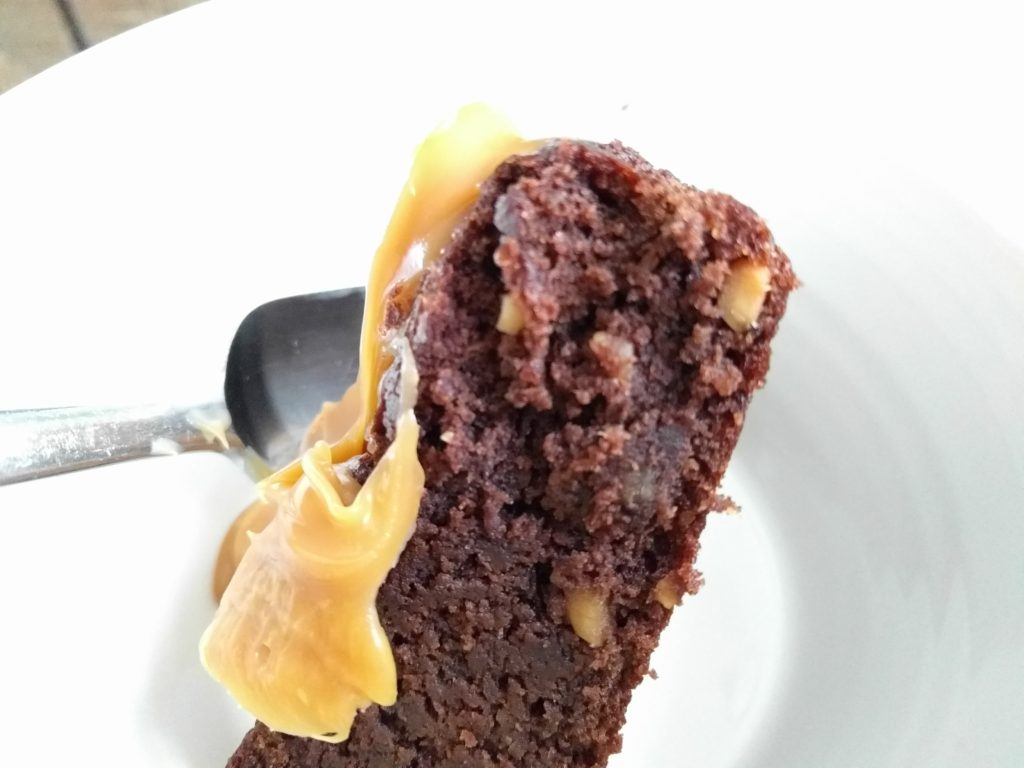
\includegraphics[width=.9\textwidth]{images/AIcake.jpg}

	{\tiny \href{http://ellis.scot/2017/05/baking-with-a-recipe-written-by-a-neural-network/}{http://ellis.scot/2017/05/baking-with-a-recipe-written-by-a-neural-network/}}
\end{frame}

\begin{frame}{How to achieve these goals}
	% no strategy is a bad strategy
	% they are just tools
	% the trick is figuring out when they are useful
	What strategy to pick given these goals? \pause
    \begin{itemize}
		\item No strategy is inherently good or bad \pause
		\item They are tools, and like any tools, the task is to figure out when and where they are useful
	\end{itemize}
\end{frame}

\begin{frame}{A general toolkit}
	Let's consider some strategies we can use for NLG: \pause

	\begin{itemize}
		\item exhaustive listing \pause
		\item rules and/or principles \pause
		\item Machine Learning \pause
	\end{itemize}

	\pause

	Where does each strategy fit best? How to combine them?
\end{frame}

\begin{frame}{Perspective}
	What do you see? How would you recreate this data distribution?
	\begin{center}
		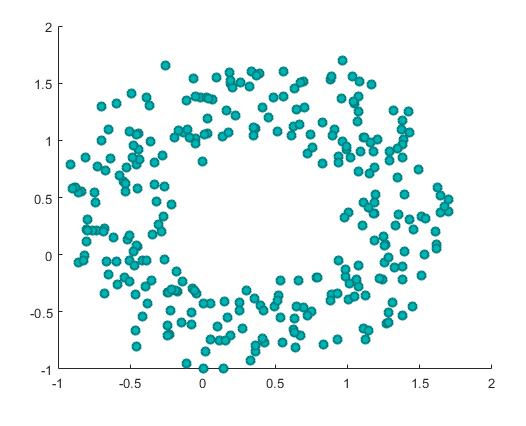
\includegraphics[width=.8\textwidth]{images/circleplot.png}
	\end{center}
\end{frame}

\begin{frame}{Outline of talk}
    % TODO this also includes "overview" and "conclusion",
    % do we need this slide at all?
	\tableofcontents
\end{frame}

%%%%%%%%%%%%%%%%%%%%%%%%%%%%%%%%%%%%%%%%%%%%%%%%%%%%%%%%%%%%%%

\section{Irregular Verbs}
\begin{frame}{Verb Inflection}
	\begin{itemize}
		\item A single verb can have various {\bf word forms}:
	\end{itemize}

	\begin{exe}
		\ex {\sc create}	\begin{xlist}
			\ex\label{createInfl} \emph{create, creates, created, creating}
			\ex\label{createDer} \emph{creator, creation, creative, creatively}
		\end{xlist}
	\end{exe}

	\begin{itemize}
		\item (\ref{createInfl}) is an example of {\bf inflectional morphology}
		\begin{itemize}
			\item expresses grammatical features
			\item (usually) doesn't change basic meaning or part of speech
		\end{itemize}
	\end{itemize}
\end{frame}

\begin{frame}{Grammatical features}
	\begin{itemize}
		\item \textbf{Grammatical features} are properties that the grammar of any language tracks and manifests
		\item Some features that English is sensitive to:
		\begin{itemize}
			\item \textbf{number}: \emph{dog, dogs}
			\item \textbf{tense}: \emph{create, created}
			\item \textbf{gender}: \emph{he, she}
			\item \textbf{person}: \emph{we, yall, they}
			\item \textbf{mass/count}: \emph{3 books, *3 bloods}
			\item \textbf{case}: \emph{I, me, my, mine}
		\end{itemize}
	\end{itemize}
\end{frame}

\begin{frame}{Inflectional Paradigms}
	\begin{itemize}
		\item Word forms can track multiple features at once
		\item This can be tracked within an \bf{inflectional paradigm}
	\end{itemize}

	\begin{table}
		{\sc create} \\
		\begin{multicols}{2}

			{\bf Present}	\\
			\begin{tabular}{|r|cc|}
				\toprule
					&	singular	&	plural	\\
				\midrule
				1	&	create 	&	create 	\\
				% \midrule
				2	&	create 	&	create 	\\
				% \midrule
				3	&	creates &	create 	\\
				\bottomrule
			\end{tabular}

			{\bf Past}	\\
			\begin{tabular}{|r|cc|}
				\toprule
					&	singular	&	plural	\\
				\midrule
				1	&	created 	&	created 	\\
				% \midrule
				2	&	created 	&	created 	\\
				% \midrule
				3	&	created &	created 	\\
				\bottomrule
			\end{tabular}
		\end{multicols}
	\end{table}
	\pause

	% Clayton

	\begin{itemize}
		\item Only 3rd person singular is different -- this looks easy!
		\begin{itemize}
			\item Just add \alert{-s} to the 3.sg present form and \alert{-d} to all past forms!
		\end{itemize}
	\end{itemize}
\end{frame}


\begin{frame}{Irregulars}
	Unfortunately, we all know there are {\bf irregular verbs} in English

	\begin{table}
		{\sc be} \\
		\begin{multicols}{2}

			{\bf Present}	\\
			\begin{tabular}{|r|cc|}
				\toprule
					&	singular	&	plural	\\
				\midrule
				1	&	am 	&	are 	\\
				% \midrule
				2	&	are 	&	are 	\\
				% \midrule
				3	&	is &	are 	\\
				\bottomrule
			\end{tabular}

			{\bf Past}	\\
			\begin{tabular}{|r|cc|}
				\toprule
					&	singular	&	plural	\\
				\midrule
				1	&	was 	&	were 	\\
				% \midrule
				2	&	were 	&	were 	\\
				% \midrule
				3	&	was &	were 	\\
				\bottomrule
			\end{tabular}
		\end{multicols}
	\end{table}

	\pause

	\begin{itemize}
		\item Darn, how do we get \alert{am} or \alert{was} from \alert{be}?
	\end{itemize}
\end{frame}

\begin{frame}{Best strategy}
	% Ok, so what strategy should we try to apply?
	Irregular verbs are arbitrary and follow no underlying pattern
	\pause
	\begin{itemize}
		\item exhaustive listing
		\item rules and/or principles
		\item Machine Learning
	\end{itemize}

\end{frame}

\begin{frame}{Finite problem set}
	\begin{itemize}
		\item Wikipedia lists about 200 English irregular verbs
		\begin{itemize}
			\item including \alert{shrive}, \alert{stave}, \alert{gild}
		\end{itemize}
		\item This is a finite set%, and most words aren't even that relevant
		% \item Verb dictionaries exist
		% \item There are subgroups within the irregulars
		% \item feasible to hardcode a list of all irregulars %without rules or ML
		% \item We can exactly fit the data without over- or undergeneralizing
		\item Prediction is not important
	\end{itemize}
\end{frame}

%%%%%%%%%%%%%%%%%%%%%%%%%%%%%%%%%%%%%%%%%%%%%%%%%%%%%%%%%%%%%

% Mike
\section{Pronouns}
\begin{frame}{Anaphora}
	\begin{description}
		\item[Anaphora] Expressions that depend on a contextual antecedent for their interpretation
		\item[Pronoun] A type of anaphor that can replace a \textbf{Noun Phrase (NP)} (or Determiner Phrase)
	\end{description}

	\begin{table}
		\begin{multicols}{2}

			{\bf Nominative}	\\
			\begin{tabular}{|r|cc|}
				\toprule
					&	singular	&	plural	\\
				\midrule
				1	&	I 	&	we 	\\
				% \midrule
				2	&	you 	&	you/yall/yinz 	\\
				% \midrule
				3	&	she/he/it &	they 	\\
				\bottomrule
			\end{tabular}

			{\bf Accusative}	\\
			\begin{tabular}{|r|cc|}
				\toprule
					&	singular	&	plural	\\
				\midrule
				1	&	me 	&	us 	\\
				% \midrule
				2	&	you 	&	you/yall/yinz 	\\
				% \midrule
				3	&	her/him/it &	them 	\\
				\bottomrule
			\end{tabular}
		\end{multicols}
	\end{table}
\end{frame}

\begin{frame}{Entity reference}
	\begin{quote}
		In later years, holding forth to an interviewer or to an audience of aging fans at a comic book convention, Sam Clay liked to declare, apropos of \textbf{his} and Joe Kavalier's greatest creation, that back when \textbf{he} was a boy, sealed and hog-tied inside the airtight vessel known as Brooklyn, New York, \textbf{he} had been haunted by dreams of Harry Houdini. "To \textbf{me}, Clark Kent in a phone booth and Houdini in a packing crate, \textbf{they} were one and the same thing,"[...]

		% \pause
		\medskip
		-Michael Chabon, The Amazing Adventures of Kavalier \& Clay
	\end{quote}

	\pause

	\begin{itemize}
		\item Connecting reference between expressions is non-trivial!
	\end{itemize}
\end{frame}

\begin{frame}{Entity reference: no ambiguity}
	\begin{quote}
		In later years, holding forth to an interviewer or to an audience of aging fans at a comic book convention, Sam Clay liked to declare, apropos of \textbf{Sam Clay} and Joe Kavalier's greatest creation, that back when \textbf{Sam Clay} was a boy, sealed and hog-tied inside the airtight vessel known as Brooklyn, New York, \textbf{Sam Clay} had been haunted by dreams of Harry Houdini. "To \textbf{Sam Clay}, Clark Kent in a phone booth and Houdini in a packing crate, \textbf{Clark Kent and Houdini} were one and the same thing,"[...]

		% \pause
		\medskip
		-Michael Chabon, The Amazing Adventures of Kavalier \& Clay: The pronoun-less edition
	\end{quote}

	\begin{itemize}
		\item Using unambiguous reference sounds clunky and un-human \pause
		\item Like the system has no idea what it's talking about
	\end{itemize}
\end{frame}

\begin{frame}{Entity reference: no ambiguity}
	\begin{center}
		
\includegraphics[width=.8\textwidth]{images/zelda.jpg}
	\end{center}
\end{frame}

\begin{frame}{Picking a strategy}
	\begin{itemize}
		\item Strawman argument: hardcoding every possible instance to use a pronoun is out 	\pause
		\item Machine Learning? \pause Is likely possible...	\pause
		\begin{itemize}
			\item what are the features we want to track?
			\item how arbitrary is the data?
		\end{itemize}
		\pause
		\item "Though this be madness, yet there is method in 't."
	\end{itemize}
\end{frame}

% Clayton
\begin{frame}{A principled approach}
	\begin{itemize}
		\item The distribution of pronouns is not arbitrary
		\item We actually probably have a pretty good idea of when we can use pronouns \pause
		\item They seem to \textbf{corefer} with recently mentioned entities that match their description \pause
		\item Let's try a rule:
	\end{itemize}

	\begin{exe}
		\ex \textbf{Pronoun Rule 1}: If the entity is the same as the most recent entity with the same \textbf{features} (person, gender, number), a pronoun can be used
	\end{exe}
\end{frame}

\begin{frame}{Does it work?}
	\begin{exe}
		\ex \begin{xlist}
			\ex Harry was in Gryffindor.
			\ex \textbf{He} was friends with Ron.
			\ex\label{prorulefail} \textbf{He} had a pet rat.
		\end{xlist}
	\end{exe}

	\begin{itemize}
		\item Who does \alert{He} in (\ref{prorulefail}) refer to? Harry or Ron? \pause
		\item Ron is the most recent singular masculine entity
		\item so why doesn't \alert{He} corefer? \pause
		\item It seems like linear order is too simplistic of an approach
	\end{itemize}
\end{frame}

\begin{frame}{Saliency}
	\begin{itemize}
		\item Pronouns (across sentences) are tracking \textbf{saliency}
	\end{itemize}

	\begin{description}
		\item[Salient:] assumed to be in the \textbf{addressee}'s consciousness at the \textbf{utterance time} \pause
	\end{description}

	\begin{exe}
		\ex Harry studies at Hogwarts with Ron.
	\end{exe}

	\begin{itemize}
		\item Who is more salient? Harry? or Ron? \pause
		\item Why?
	\end{itemize}
\end{frame}

\begin{frame}{Information structure}
	\Tree
		[.S
			[.NP \textbf{Harry} ][.VP
				[.VP
					[.VP
						[.V studies ]
					][.PP
						[.P at ][.NP Hogwarts ]
					]
				][.PP
					[.P with ][.NP \textbf{Ron} ]
				]
			]
		]

	\begin{itemize}
		\item Subjects are structurally higher than objects
		\item In English this correlates with saliency
	\end{itemize}

\end{frame}
\begin{frame}{Tracking saliency}
	An advanced NLG system should track saliency in order to use pronouns
	\begin{itemize}
		\item Pronoun distribution is based on known principles
		\item The AI system should also share those principles \vspace{10pt}
		 \pause

		\item Syntactic structure strongly influences saliency
		\item We can use Quill's understanding of a sentence's underlying
			structure to emulate this linguistic phenomenon
	\end{itemize}
\end{frame}

\begin{frame}{Other factors?}
	\begin{itemize}
		\item But are there other factors at play? \pause
		\begin{itemize}
			\item recency
			\item repetition
			\item ?? \pause
		\end{itemize}
		\item How would these interact with each other?
	\end{itemize}
\end{frame}

%%%%%%%%%%%%%%%%%%%%%%%%%%%%%%%%%%%%%%%%%%%%%%%%%%%%%%%%%%%%%%%%%%%

\section{Sentence Selection}
\begin{frame}{Variability}
    A typical Quill sentence:
    \begin{exe}
        \ex \begin{xlist}
            \ex Aaron Young generated \$3M in revenue in 2016. \\ \pause
            \ex Aaron Young's revenue was \$3M in 2016.
            \ex Revenue for Aaron Young was \$3M in 2016.
            \ex In 2016, Aaron Young generated \$3M in revenue.
            \ex Aaron Young's 2016 generated revenue was \$3M.
        \end{xlist}
    \end{exe}
\end{frame}

\begin{frame}{Grammaticality vs Style}
    \begin{description}
        \item[Sentece generation:] only grammatical and accurate sentences should be {\bf generated}
        \item[Sentence selection:] the stylistically best sentence from the set of grammatical candidate sentences should be {\bf selected} \pause
    \end{description}

    \begin{itemize}
        \item but what determines a stylistically `good` sentence?
    \end{itemize}
\end{frame}

\begin{frame}{What makes a good sentence?}
    \begin{itemize}
        \item Most native speakers will agree when a sentence is grammatical
        \item But style is vague and elusive, varying from person to person   \pause
        \item Which do think is the best sentence?
    \end{itemize}

    \begin{exe}
    	\ex \begin{xlist}
	        \ex Aaron Young generated \$3M in revenue in 2016.
	        \ex Aaron Young's revenue was \$3M in 2016.
	        \ex Revenue for Aaron Young was \$3M in 2016.
	        \ex In 2016, Aaron Young generated \$3M in revenue.
	        \ex Aaron Young's 2016 generated revenue was \$3M.
	    \end{xlist}
    \end{exe}

    \pause
    \begin{itemize}
    	\item is there even a right answer?
    \end{itemize}
\end{frame}

\begin{frame}{Multiple axes of 'goodness'}
	\begin{itemize}
		\item There seem to be multiple factors involved:
		\begin{itemize}
			\item length
			\item subject choice
            % Not relevant to this example, might be confusing
			%\item values before attributes
			\item fronted information
			\item strong verbs vs copulas
			\item ...	\pause
		\end{itemize}
		\item These axes seem largely independent
	\end{itemize}
\end{frame}

\begin{frame}{Extensibility}
	\begin{itemize}
		\item Hand-tuning sentence selection got unscaleable as the complexity
            and breadth of possible sentences in the system increased
		\item Humans are bad at keeping track of all possible permutations of interactions \pause
		\begin{itemize}
			\item Maybe we prefer active vs passive verbs, but what if that results in longer sentences? \pause
		\end{itemize}
		\item Different users also vary in how strongly they weight each factor
	\end{itemize}
\end{frame}

\begin{frame}{Did somebody say "weight"?}
	\begin{itemize}
		\item Interaction of multiple features %Sentence selection involves the interaction between several features
		\item Features have varying importance %The importance of these features is variable
		\item Importances should be tuneable \pause %We would like to fine tune language style for each user \pause
		\item This feels like a job for Machine Learning
	\end{itemize}
\end{frame}

\begin{frame}{Let the machine figure out what matters}
	Steps to utilizing Machine Learning for sentence selection:

	\begin{itemize}
		\item Determine list of features that matter for style
		\item Build independent weighers for features
		\item Collect data
		\item Train the model on the data with respect to the features
		\item Use the model to select the best candidate sentence
		\item Lather, rinse, repeat
	\end{itemize}
\end{frame}

% \begin{frame}{Tunability}
% 	\begin{itemize}
% 		\item While grammaticality is essentially uniform, style varies
% 		\item Trying to hand-tune sentence-selection for each user would be difficult	\pause
% 		\begin{itemize}
% 			\item how to make a change in one place without breaking it elsewhere?	\pause
% 		\end{itemize}
% 		\item Given an ML model, we can retrain the feature weights for each user or domain
% 	\end{itemize}
% \end{frame}

\begin{frame}{Finally, just throw ML at it}

	\begin{itemize}
		\item Machines are great at working with these independent features
		\item Humans are still responsible for building out each new feature\pause
	\end{itemize}
    While the core decision is an ML problem, the inputs to that
    decision are still based on linguistic principles

\end{frame}


\begin{frame}{Lessons and caveats}
	\begin{itemize}
		\item Machine Learning is a good strategy for sentence selection
		\item Style is variable and involves the interaction between several features \pause
		\item \alert{Caveat:} We need to be able to determine those features and how to track them
		\begin{itemize}
			\item which often requires an understanding of the domain
		\end{itemize}
	\end{itemize}
\end{frame}

%%%%%%%%%%%%%%%%%%%%%%%%%%%%%%%%%%%%%%%%%%%%%%%%%%%%%%%%%%%%%%%%%%%

% Mike
\section{Conclusion}
\begin{frame}{Perspectives redux}
	What do you see?
	\begin{center}
		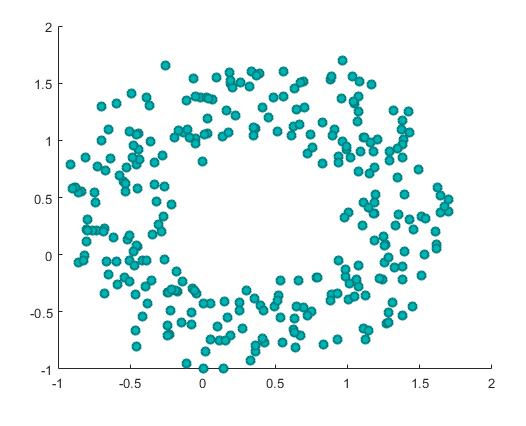
\includegraphics[width=.6\textwidth]{images/circleplot.png}
	\end{center}

	\pause
	\begin{itemize}
		\item \textbf{Irregular verbs:} discrete points	\pause
		\item \textbf{Pronouns}: conceptual circle $\rightarrow$ messy data	\pause
		\item \textbf{Sentence selection}: messy data $\rightarrow$ conceptual circle
	\end{itemize}
\end{frame}

\begin{frame}{Chimerical problems}
	Problems are often multi-faceted:

	\begin{itemize}
		\item Verb inflection does have regular rules
		\item Antecedent saliency for pronominal reference may have multiple factors
		\item Sentence selection features require principled analysis
	\end{itemize}
\end{frame}

\begin{frame}{Chimerical solutions}
	Things we've learned creating advanced NLG:

	\begin{itemize}
		\item Strategies for tackling problems should not (always) be monolithic
		\item Utilize whatever tools you have	\pause
		\item but make sure those strategies are contingent on thoroughly assessing the nature of the problems \pause
		\item which often requires having domain knowledge \pause
		\begin{itemize}
			\item go learn about what others have done in your field \pause
			\item from various perspectives: e.g. linguistics, comp sci, journalism,\ldots
		\end{itemize}
	\end{itemize}
\end{frame}

\plain{}{Thank you! \\ Questions?}


% \begin{frame}[fragile]
%   \frametitle{mtheme}

%   The \emph{mtheme} is a Beamer theme with minimal visual noise inspired by the
%   \href{https://github.com/hsrmbeamertheme/hsrmbeamertheme}{\textsc{hsrm} Beamer
%   Theme} by Benjamin Weiss.

%   Enable the theme by loading

%   \begin{minted}[fontsize=\small]{latex}
%     \documentclass{beamer}
%     \usetheme{m}
%   \end{minted}

%   Note, that you have to have Mozilla's \emph{Fira Sans} font and XeTeX
%   installed to enjoy this wonderful typography.
% \end{frame}

% \begin{frame}[fragile]
%   \frametitle{Sections}
%   Sections group slides of the same topic

%   \begin{minted}[fontsize=\small]{latex}
%     \section{Elements}
%   \end{minted}

%   for which the \emph{mtheme} provides a nice progress indicator \ldots
% \end{frame}

% \section{Elements}

% \begin{frame}[fragile]
%   \frametitle{Typography}
%       \begin{minted}[fontsize=\small]{latex}
% The theme provides sensible defaults to \emph{emphasis}
% text, \alert{accent} parts or show \textbf{bold} results.
%       \end{minted}

%   \begin{center}becomes\end{center}

%   The theme provides sensible defaults to \emph{emphasis} text,
%   \alert{accent} parts or show \textbf{bold} results.
% \end{frame}

% \begin{frame}{Lists}
%   \begin{columns}[onlytextwidth]
%     \column{0.5\textwidth}
%       Items
%       \begin{itemize}
%         \item Milk \item Eggs \item Potatos
%       \end{itemize}

%     \column{0.5\textwidth}
%       Enumerations
%       \begin{enumerate}
%         \item First, \item Second and \item Last.
%       \end{enumerate}
%   \end{columns}
% % \end{frame}

% \begin{frame}{Descriptions}
%   \begin{description}
%     \item[PowerPoint] Meeh.
%     \item[Beamer] Yeeeha.
%   \end{description}
% \end{frame}

% \begin{frame}{Animation}
%   \begin{itemize}[<+- | alert@+>]
%     \item \alert<4>{This is\only<4>{ really} important}
%     \item Now this
%     \item And now this
%   \end{itemize}
% \end{frame}

% \begin{frame}{Figures}
%   \begin{figure}
%     \newcounter{density}
%     \setcounter{density}{20}
%     \begin{tikzpicture}
%       \def\couleur{mLightBrown}
%       \path[coordinate] (0,0)  coordinate(A)
%                   ++( 90:5cm) coordinate(B)
%                   ++(0:5cm) coordinate(C)
%                   ++(-90:5cm) coordinate(D);
%       \draw[fill=\couleur!\thedensity] (A) -- (B) -- (C) --(D) -- cycle;
%       \foreach \x in {1,...,40}{%
%           \pgfmathsetcounter{density}{\thedensity+20}
%           \setcounter{density}{\thedensity}
%           \path[coordinate] coordinate(X) at (A){};
%           \path[coordinate] (A) -- (B) coordinate[pos=.10](A)
%                               -- (C) coordinate[pos=.10](B)
%                               -- (D) coordinate[pos=.10](C)
%                               -- (X) coordinate[pos=.10](D);
%           \draw[fill=\couleur!\thedensity] (A)--(B)--(C)-- (D) -- cycle;
%       }
%     \end{tikzpicture}
%     \caption{Rotated square from
%     \href{http://www.texample.net/tikz/examples/rotated-polygons/}{texample.net}.}
%   \end{figure}
% \end{frame}

% \begin{frame}{Tables}
%   \begin{table}
%     \caption{Largest cities in the world (source: Wikipedia)}
%     \begin{tabular}{lr}
%       \toprule
%       City & Population\\
%       \midrule
%       Mexico City & 20,116,842\\
%       Shanghai & 19,210,000\\
%       Peking & 15,796,450\\
%       Istanbul & 14,160,467\\
%       \bottomrule
%     \end{tabular}
%   \end{table}
% \end{frame}
% \begin{frame}{Blocks}

%   \begin{block}{This is a block title}
%     This is soothing.
%   \end{block}

% \end{frame}
% \begin{frame}{Math}
%   \begin{equation*}
%     e = \lim_{n\to \infty} \left(1 + \frac{1}{n}\right)^n
%   \end{equation*}
% \end{frame}
% \begin{frame}{Quotes}
%   \begin{quote}
%     Veni, Vidi, Vici
%   \end{quote}
% \end{frame}

% \plain{Dark background}{\vspace{-2em}\begin{center}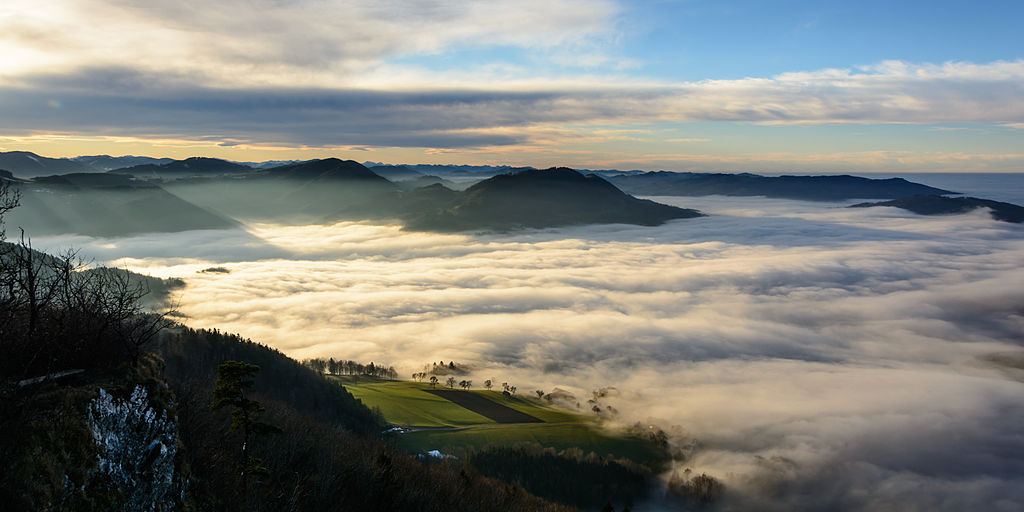
\includegraphics[width=\textwidth]{images/valley.jpg}\end{center}}


\begin{frame}{Beamer theme}

  Get the source of this theme and the demo presentation from

  \begin{center}\url{github.com/matze/mtheme}\end{center}

  The theme \emph{itself} is licensed under a
  \href{http://creativecommons.org/licenses/by-sa/4.0/}{Creative Commons
  Attribution-ShareAlike 4.0 International License}.

  \begin{center}\ccbysa\end{center}

\end{frame}

% \plain{}{Questions?}

\end{document}
